\CourseSection{Functional Description}\label{sec:functional-description}
\CourseSubsection{System overview}

\Guidance{Use a set of diagrams to explain the system boundary, internal functions, operating behavior, inputs and outputs, signal types, protocols, direction of information flow, computing architecture, and / or anything else that applies. Write a short paragraph here that explains design decisions and references each figure, like Figure~\ref{fig:system}. Maintain labeling consistency (such as IDs, components, units, etc.) across tables and figures in this document. It's a good idea to reference these later in Section~\ref{sec:testing}.}
The system architecture is organized into functional, physical, and logical domains to validate core autonomous mobility, safety, and equipment auditing without unnecessary complexity. Figure~\ref{fig:functional-architecture} outlines the primary operational blocks, showing energy and signal paths between tracking, obstacle detection, club monitoring, and motor drive systems. Figure~\ref{fig:physical-layout} defines the physical component distribution and interface boundaries across the chassis, emphasizing sensor clearance and immediate access to safety overrides (\textbf{IF-02}). Finally, Figure~\ref{fig:logical-architecture} details the logical execution stack and hardware communication protocols (UART, SPI, I2C, and GPIO interrupts), prioritizing deterministic low-latency handling for emergency stop triggers (\textbf{PF-05}).

\begin{figure}[htbp]
\centering
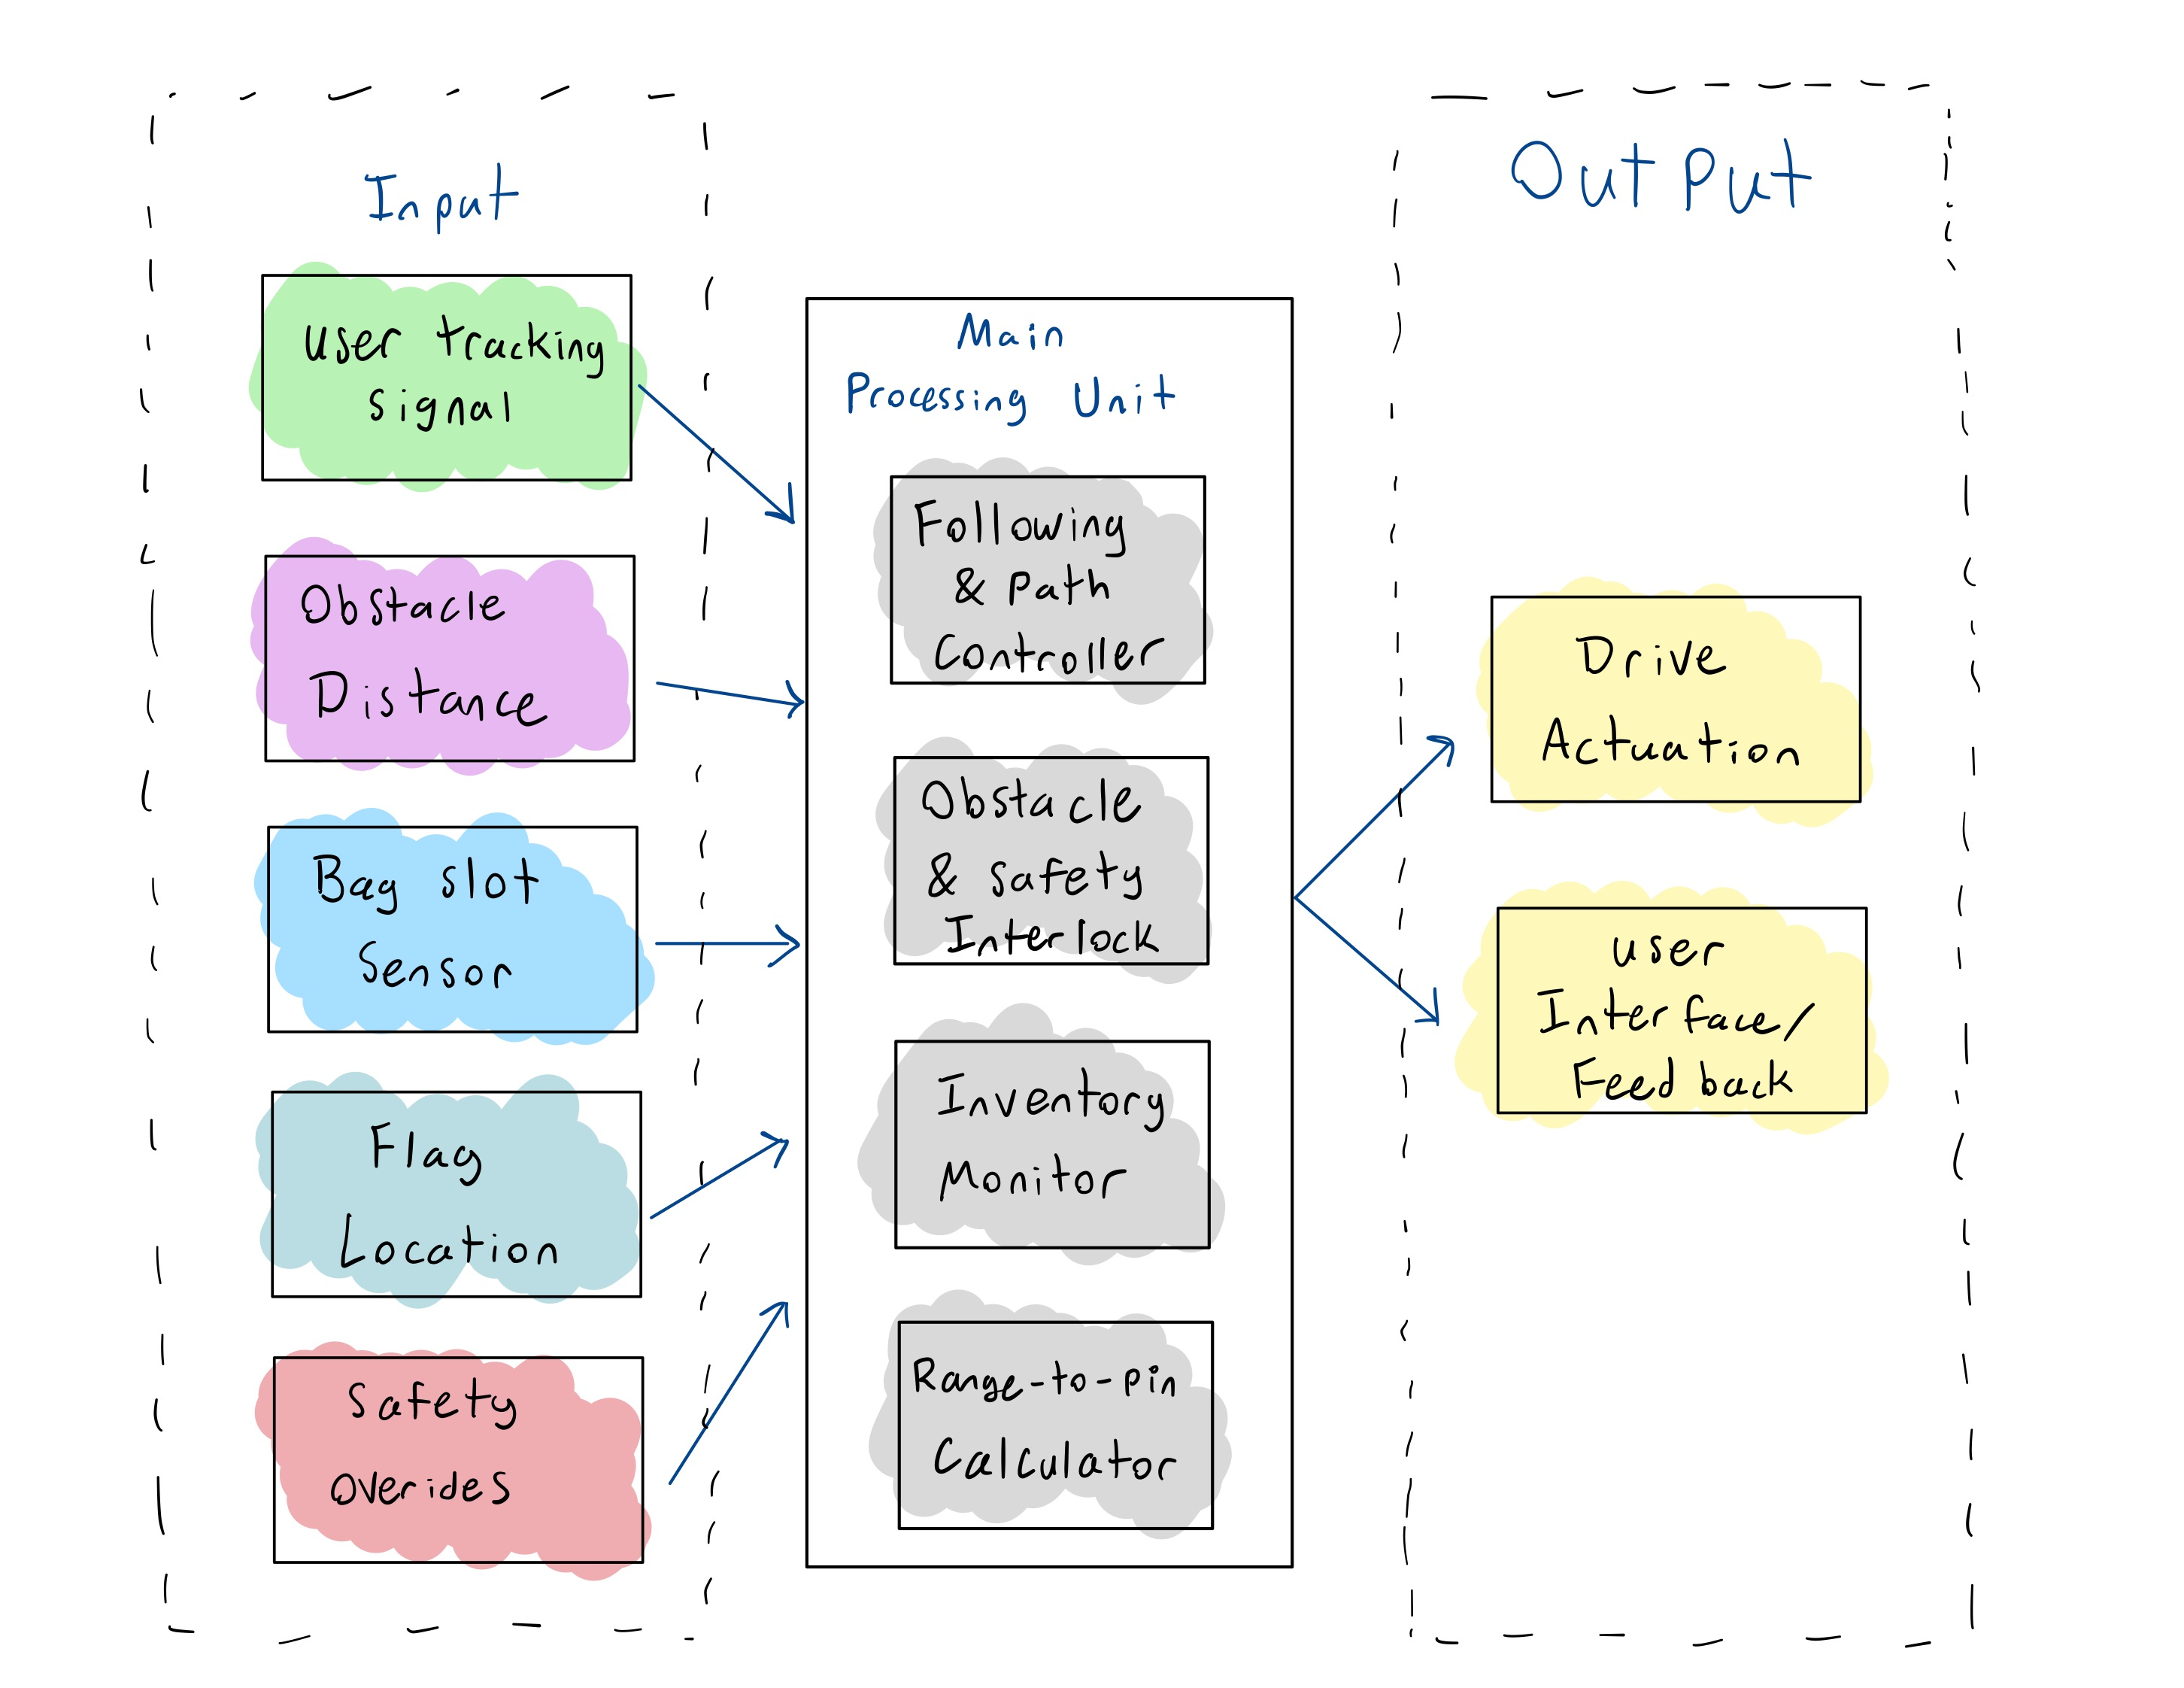
\includegraphics[width=0.9\linewidth]{figures/functional.jpeg}
\caption{Functional architecture diagram showing inputs, processing interlocks, and control outputs for the MVP smart caddy system.}
\label{fig:functional-architecture}
\end{figure}

\begin{figure}[htbp]
\centering
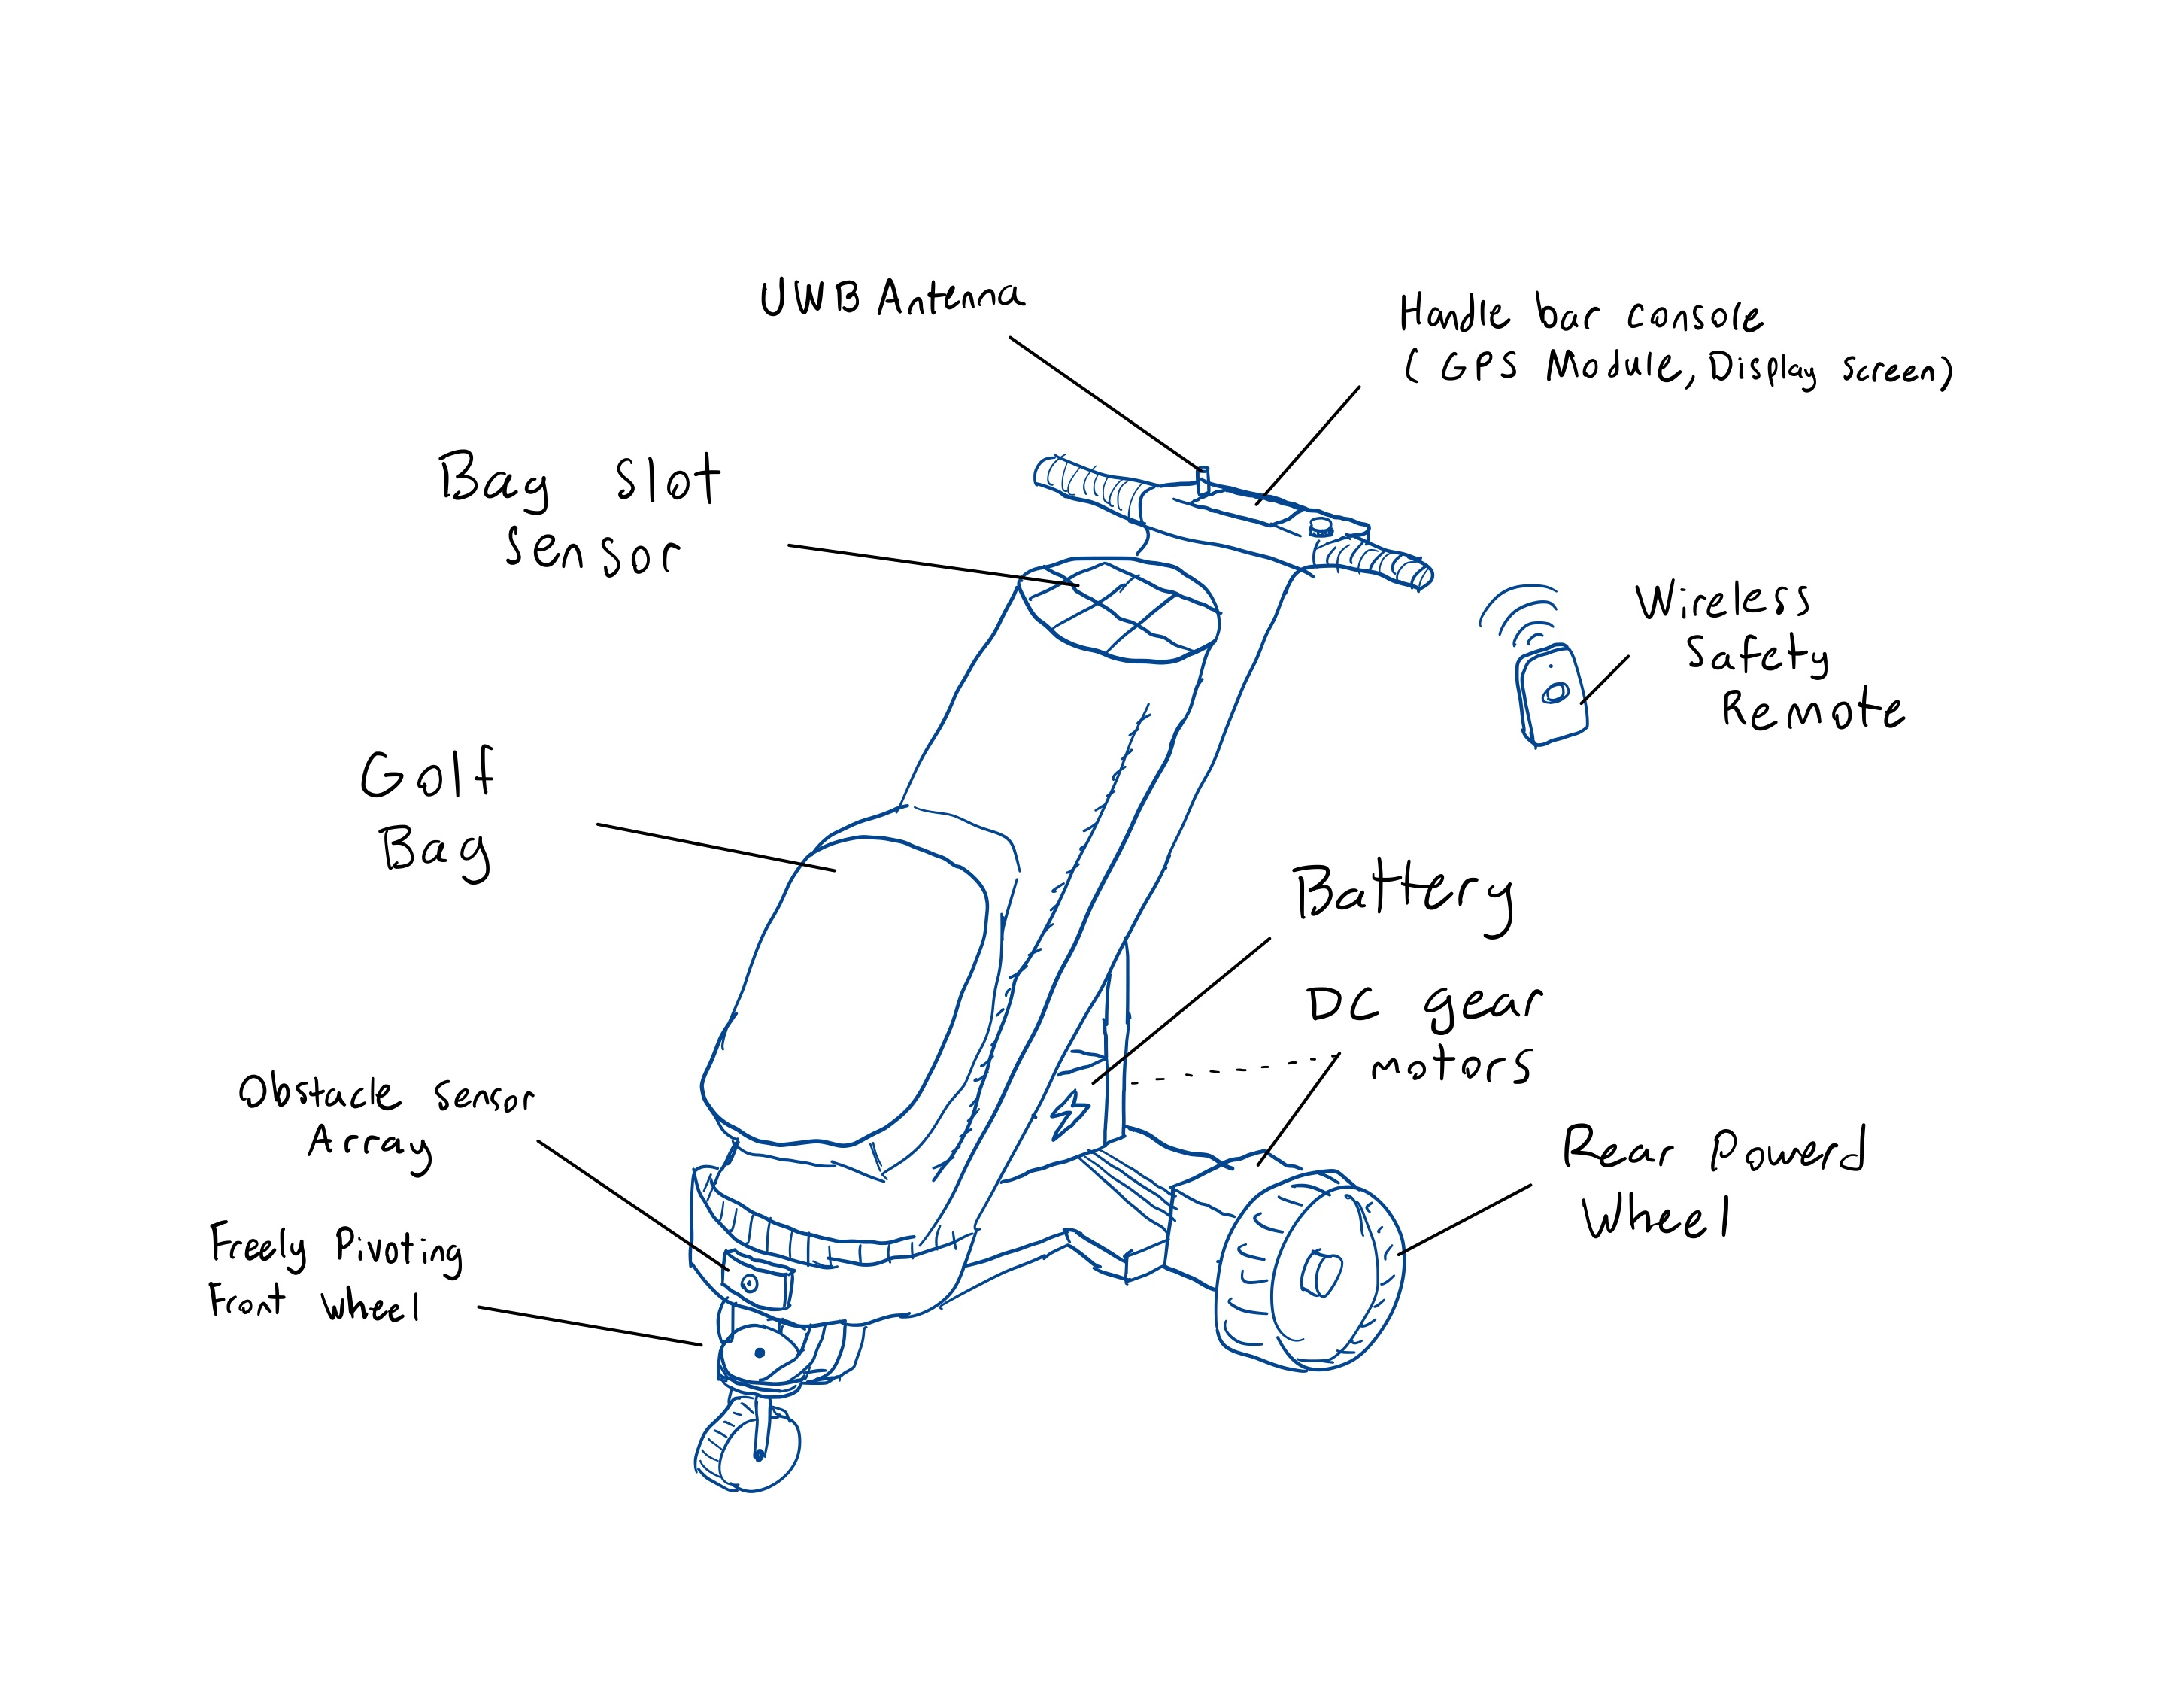
\includegraphics[width=0.9\linewidth]{figures/physical.jpeg}
\caption{Physical layout diagram detailing component placement, structural enclosures, bag cradle sensors, and safety controls on the chassis.}
\label{fig:physical-layout}
\end{figure}

\begin{figure}[htbp]
\centering
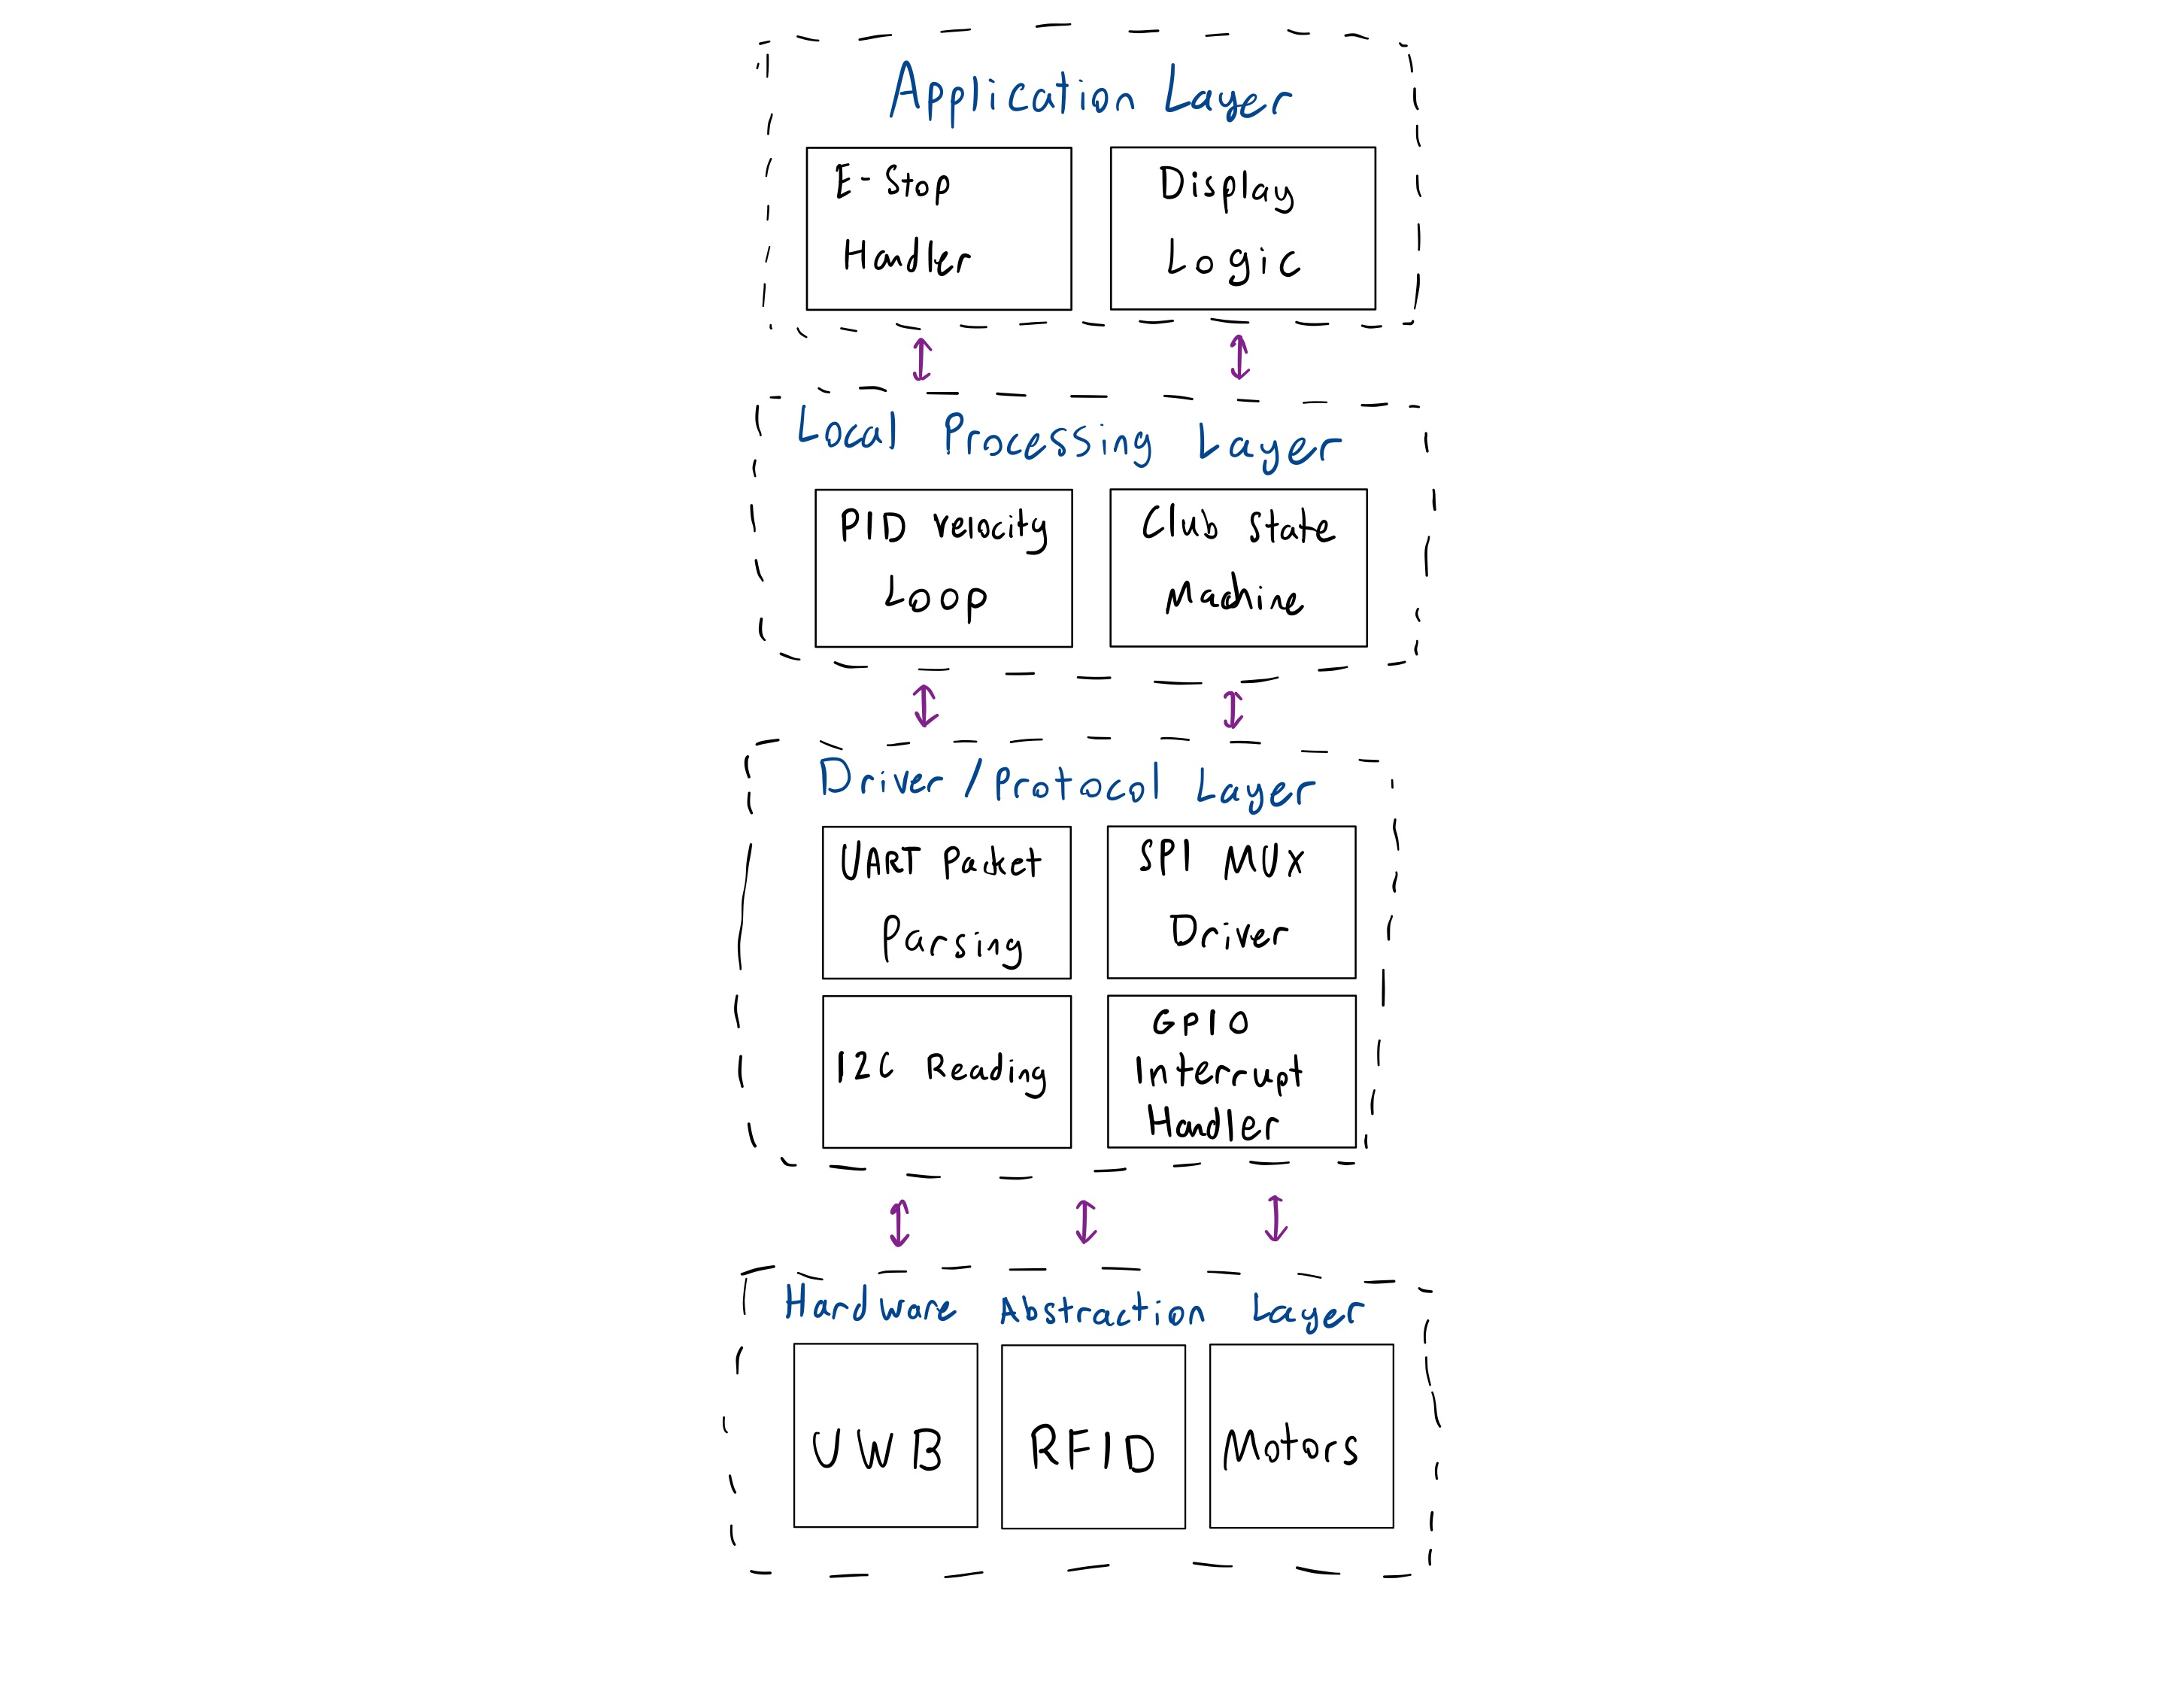
\includegraphics[width=0.9\linewidth]{figures/logical.jpeg}
\caption{Logical computing architecture outlining the hardware abstraction layer, driver protocols, logical processing loops, and low-latency safety interrupts.}
\label{fig:logical-architecture}
\end{figure}

\clearpage
\CourseSubsection{Interface and performance specifications}
\Guidance{Give quantitative targets and tolerances with proper units. You can also use IDs to connect specifications with the tests in Section~\ref{sec:testing}. Write a short paragraph here giving context for these requirements, citing the IDs as necessary.}
The interface and performance specifications defined in Table~\ref{tab:proposal-specs} establish the measurable quantitative targets required to ensure the smart caddy effectively alleviates physical strain and cognitive load for senior golfers. Physical and hardware interfaces focus on ergonomic accessibility, payload capacity, and reliable user tracking (\textbf{IF-01} through \textbf{IF-04}). Performance metrics guarantee that the mechatronic chassis maintains safe following distances, handles standard 18-hole course topographies, and reliably detects active club removal and return (\textbf{PF-01} through \textbf{PF-05}). Each specification is tagged with a unique identifier to facilitate downstream verification and validation in Section~\ref{sec:testing}.

\begin{singlespace}
\setlength{\LTcapwidth}{\linewidth}
\begin{longtable}{@{}L{0.10\linewidth} L{\dimexpr0.4700000\linewidth-6.0000000\tabcolsep\relax} L{0.22\linewidth} L{0.21\linewidth}@{}}
\caption{Preliminary system specifications.}\label{tab:proposal-specs}\\
\rowcolor{MidGray}
\TableHeader{ID} & \TableHeader{Requirement} & \TableHeader{Target} & \TableHeader{Tolerance} \\
\midrule
\endfirsthead
\rowcolor{MidGray}
\TableHeader{ID} & \TableHeader{Requirement} & \TableHeader{Target} & \TableHeader{Tolerance} \\
\midrule
\endhead
\bottomrule
\endfoot
% Add and replace data rows below.
% Interface Specifications
% Interface Specifications
IF-01 & User Tracking Beacon Range & 15.0 m & $\pm$ 2.0 m \\
\addlinespace[3pt]
IF-02 & Distance-to-Flag GPS Accuracy & 3.0 m & $\le$ 5.0 m \\
\addlinespace[3pt]
IF-03 & Bag Slot Sensor Audit Resolution & 14 slots & Binary (Present/Absent) \\
\addlinespace[3pt]
IF-04 & Emergency Stop Wireless Link Range & 30.0 m & Minimum 20.0 m \\
\addlinespace[3pt]
IF-05 & Onboard Status Display Diagonal Size & 7.0 in & Minimum 5.0 in \\
\addlinespace[3pt]

% Performance Specifications
PF-01 & Obstacle Auto-Stop Reaction Time & 200 ms & $\le$ 300 ms \\
\addlinespace[3pt]
PF-02 & Maximum Autonomous Cruise Speed & 5.0 km/h & $\pm$ 0.5 km/h \\
\addlinespace[3pt]
PF-03 & Target Following Distance & 1.5 m & $\pm$ 0.3 m \\
\addlinespace[3pt]
PF-04 & Continuous Operating Distance (Single Charge) & 10.0 km & $\pm$ 1.5 km \\
\addlinespace[3pt]
PF-05 & Emergency Stop Override Latency & 50 ms & $\le$ 100 ms \\
\end{longtable}
\end{singlespace}

\CourseSubsection{Risks and safety hazards}
\Guidance{Identify relevant technical risks, health risks, and / or safety hazards, and indicate how you will manage these risks, and / or explain how system features and operating conditions are low-risk.}
\clearpage
